\newpage
\section{El problema}\label{sec:problema}

Un yacimiento petrol\'\i fero es una acumulaci\'on natural de hidrocarburos (gas natural y petr\'oleo, entre otros) en el subsuelo. Debido a la creciente escasez de reservas de hidrocarburos acumulados en yacimientos convencionales, la industria del petr\'oleo y diversos gobiernos nacionales han tornado su atenci\'on en las \'ultimas d\'ecadas a la explotaci\'on de yacimientos no convencionales. Uno de los tipos de yacimientos m\'as explorados est\'a dado por las reservas de petr\'oleo y gas natural almacenados en un tipo de rocas sedimentarias llamadas pelitas (shale), conocidos como yacimientos de \emph{shale gas} y \emph{shale oil}.
 
La explotaci\'on de este tipo de yacimientos utiliza m\'etodos de fractura hidr\'aulica, por medio de los cuales se generan fracturas en la roca madre para concentrar el petr\'oleo y el gas natural y posteriormente proceder a su extracci\'on. A pesar de que las primeras inyecciones de material para la extracci\'on de hidrocarburos se remontan a la segunda mitad del siglo XIX, reci\'en se comenz\'o a usar este tipo de m\'etodos en forma extensiva a prin\-ci\-pios del siglo XXI, principalmente en Estados Unidos. Adem\'as de las reservas en Estados Unidos, en la \'ultima d\'ecada se han descubierto enormes reservas de shale gas y shale oil en Argentina, Canad\'a y China.

Se describe el proceso de explotaci\'on de un yacimiento \emph{shale}. En primer lugar, se realizan varias perforaciones verticales en el subsuelo que llegan hasta la roca madre. Como se ve a continuacion:

\begin{center}
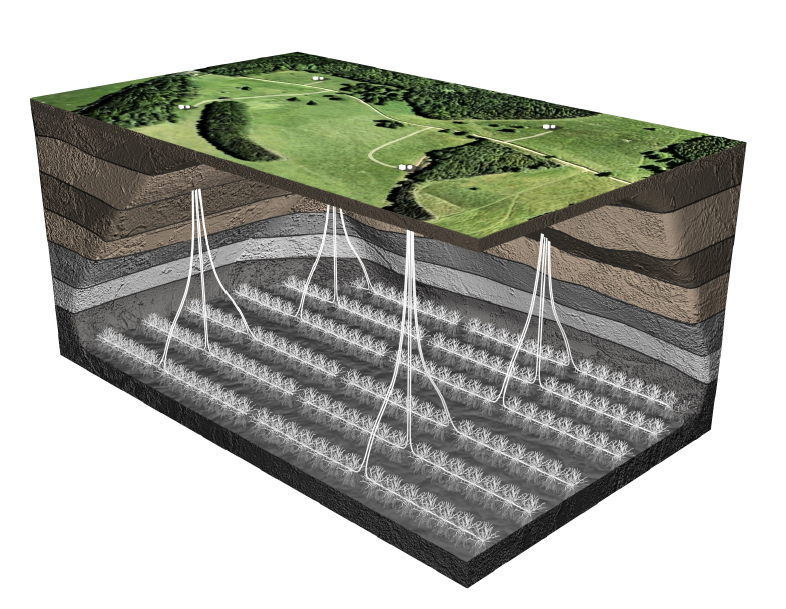
\includegraphics[width=0.5\textwidth]{imagenes/figura1}
\end{center}

\newpage
El sector en la superficie alrededor de las bocas de pozo se denomina locacion, y habitualmente ocupa un area rectangular de entre algunas decenas y unos pocos cientos de metros por lado. Estos equipos son los unicos que se ven en la supercie, y habitualmente su instalacion involucra obras de nivelacion del suelo y construccion de caminos de acceso. Como consecuencia, las locaciones no pueden estar sobre cursos de agua, barrancos o en sitios montanosos.

\begin{center}
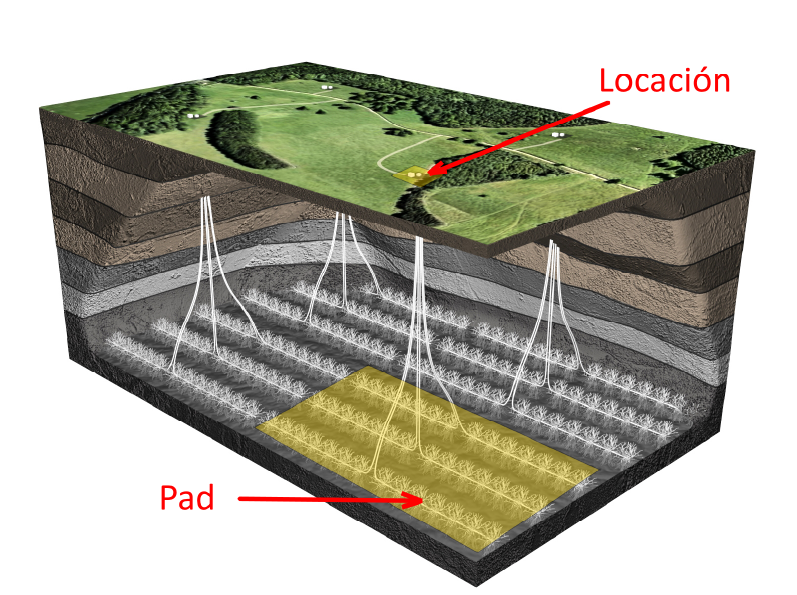
\includegraphics[width=0.4\textwidth]{imagenes/figura2}
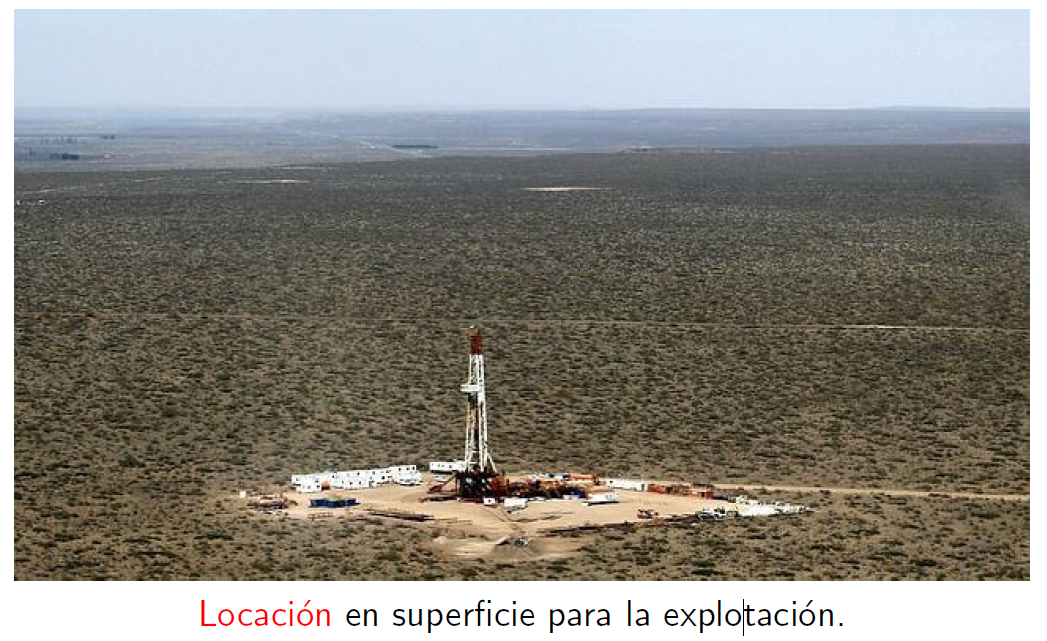
\includegraphics[width=0.4\textwidth]{imagenes/figura3}
\end{center}

Cada perforacion atraviesa la roca madre, y a lo largo de esta perforacion
se realizan los procesos de inyeccion de materiales para lograr la fractura de
la roca. Luego, se utilizan las mismas para la extraccion de los hidrocarburos
que migran hacia las zonas de fractura.

La zona
explotada a partir de una locacion se denomina pad, y tiene una forma tpicamente
rectangular.

Dadas estas caracteristicas del problemas queremos que las zonas de fractura en la roca madre no se deban superponer.


Al momento de planicar la explotacion de un yacimiento no convencional,
uno de los principales problemas a resolver es donde ubicar las locaciones y
que tipo de explotacion realizar en cada una (lo cual determina el tipo y
tamano de los pads resultantes) con el objetivo de maximizar la produccion
y minimizar los costos y el impacto ambiental. Este problema se conoce con
el nombre de optimizacion del area de drenaje, y como resultado se espera un
plan de explotacion que muestre las ubicaciones de locaciones y pads.


En la siguiente figura podemos ver  el mapa de un yacimiento, y las conguraciones de pads que
podemos usar para la explotacion.

\begin{center}
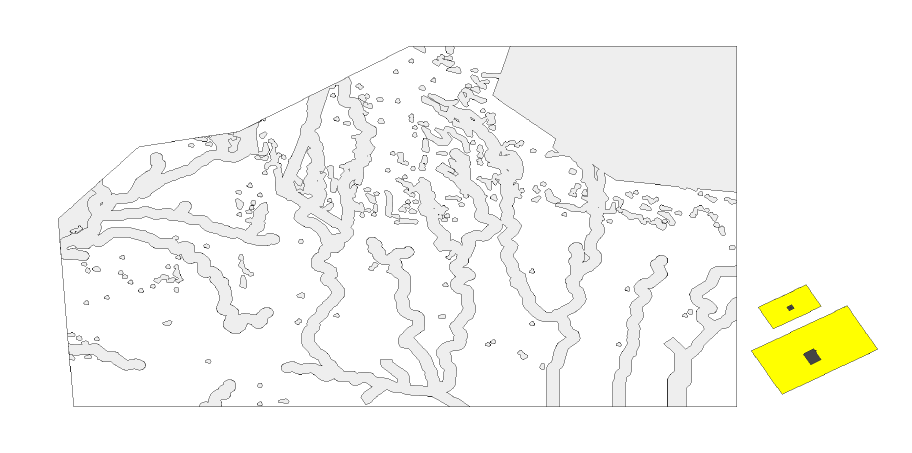
\includegraphics[width=0.4\textwidth]{imagenes/figura4}
\end{center}

Los pads se deben ubicar siguiendo cierto angulo $\alpha$, llamado direccion de esfuerzo horizontal mnimo.
Como por ejemplo:

\begin{center}
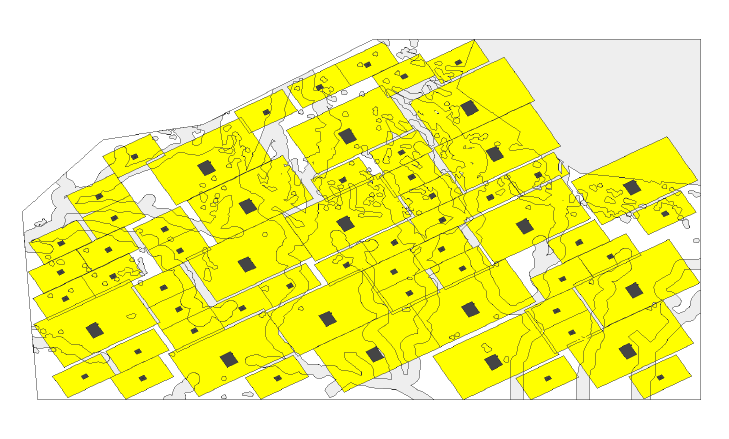
\includegraphics[width=0.4\textwidth]{imagenes/figura5}
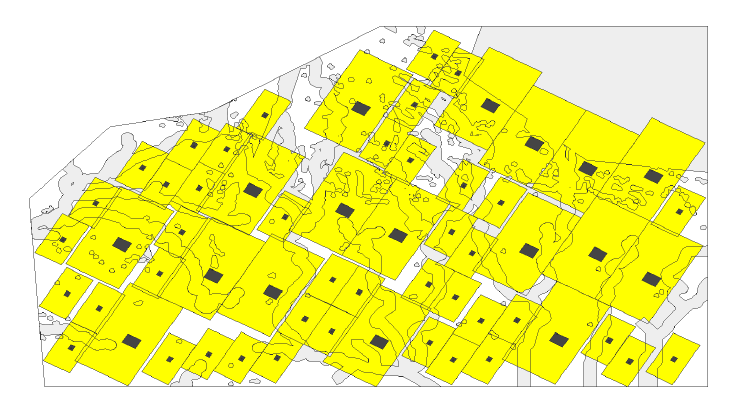
\includegraphics[width=0.4\textwidth]{imagenes/figura6}
\end{center}

Formalmente, los datos de entrada del problema estan dados por los siguientes
elementos:

\begin{enumerate}
\item El yacimiento Y  $\subseteq$ $\mathbb{R}^2$, que en este trabajo asumimos dado por un poligono en el plano (no necesariamente convexo). Todos los pads deben estar ubicados dentro del perimetro del yacimiento.
\item Una funcion ogip : Y $\rightarrow \mathbb{R}_{+}$ (original gas in place), que especica la
cantidad de shale gas esperada en cada punto del yacimiento, y el precio
de venta $\rho  \in \mathbb{R}_{+}$ de cada unidad extraida. Dado un pad P $\subseteq$ Y ubicado
dentro del yacimiento, el gas total obtenido por explotar el pad esta dado
por ogip(P) := $\int_{P}^{} ogip(x) dx$
\item Un conjunto S = \{$S_1$,...,$S_k$\} de configuraciones posibles de pads, que
podemos utilizar para explotar el yacimiento. Para cada configuracion S $\in$ S, tenemos estos datos:
\begin{enumerate}
\item  Largo $lp_S \in \mathbb{R}_{+}$ y ancho $ap_S \in \mathbb{R}_{+}$ del pad, en metros.
\item  Largo $ll_S \in \mathbb{R}_{+}$ y ancho $al_S \in \mathbb{R}_{+}$ de la locacion en metros, y asumimos que $ll_S < lp_S$ y $al_S < ap_S$.
\item  La locacion esta ubicada en el centro del pad, pero se puede mover algunos metros de este centro para evitar obstaculos geogracos. El parametro de tolerancia $tol_S \in \mathbb{R}_{+}$ especica la cantidad maxima de metros que el centro de la locacion se puede mover con relacion
al centro del pad.
\item  Finalmente, se tiene el costo $c_S \in \mathbb{R}_{+}$ de construccion del pad.
Dado un pad P correspondiente a la conguracion S, denimos su margen neto como $neto(P) := \rho$ X $ogip(P) - c_S$.
\end{enumerate}
\item  Un conjunto de obstaculos (habitualmente de indole geografica) que las locaciones deben evitar. Consideramos que cada obstaculo esta dado por un poligono en el plano, y ninguna locacion se puede superponer con ningun obstaculo.
\item Un angulo $\alpha \in [0; 2\pi]$ de explotacion ideal, denominado angulo de esfuerzo horizontal minimo, que especifica la orientacion aproximada que deben tener los pozos horizontales sobre el yacimento con relacion al norte geografico. Como esta orientacion es aproximada, se tiene una tolerancia $\beta \in [0; 2\pi]$, que especifica que todos los pads deben estar orientados en un angulo comprendido en el intervalo $[\alpha - \beta, \alpha + \beta]$.
\end{enumerate}



El problema consiste en hallar un conjunto de pads Ps = \{$P_1, ... ,P_n$\} y un conjunto de locaciones Ls = \{$L_1, ..., L_n$\} (de modo tal que la locacion $L_i$ corresponde al pad $P_i$, para i = 1,...,n) que maximice $neto(P) :=  \sum_{i=1}^{n} neto(P_i) $ de modo tal que se cumplan las siguientes restricciones:

\begin{enumerate}
\item Todos los pads deben estar contenidos dentro del yacimiento, es decir $P_i \subseteq Y$ para i = 1,...,n.
\item Como restriccion, los pads de la solucion no se deben superponer, dado que corresponden a zonas de fractura en la roca madre.
\item Cada pad y su locacion deben responder a las especicaciones de una conguracion de S. Es decir, para cada i = 1,...,n debe existir una conguracion S $\in$ S tal que $P_i$ tiene largo $lp_S$ y ancho $ap_S$, $L_i$ tiene largo $ll_S$ y ancho $al_S$ y su centro esta a no mas de $tol_S$ metros del centro de $P_i$, y finalmente $P_i$ y $L_i$ estan orientados en un mismo aangulo, el cual debe estar entre $[\alpha - \beta, \alpha + \beta]$.
\item Ninguna locacion de Ls se debe superponer con ningun obstaculo.
\end{enumerate}


Por ejemplo, en la siguiente figura se muestra un yacimiento y los obstaculos dentro del yacimiento, y en la figura contigua se muestra una solucion factible para $\alpha = \pi / 4$ y para dos configuraciones posibles. Dado que la funcion ogip no siempre esta bien determinada de antemano (y en ocasiones se trabaja con estimaciones poco fiables de esta funcion) alternativamente se puede solicitar que se maximice el area total cubierta con los pads propuestos, en lugar del benecio neto total obtenido. El algoritmo que se presenta en la proxima seccion permite utilizar cualquiera de estas dos funciones objetivo, o una combinacion lineal de ambas.



\begin{center}
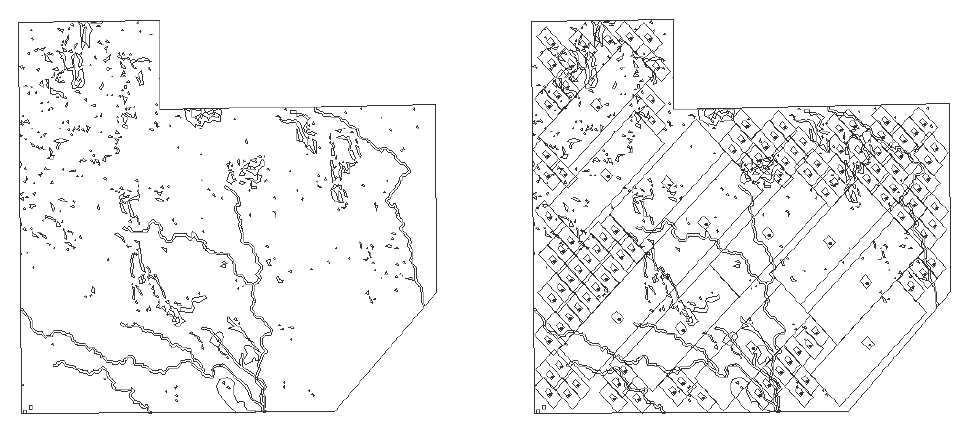
\includegraphics[width=0.7\textwidth]{imagenes/figura7}
\end{center}

